\documentclass[notitlepage]{math}
\usepackage{lipsum}
\usetikzlibrary{patterns,positioning, decorations, decorations.pathreplacing}
\title{Function Local study Chap. 10} %Titre du fichie
\author{FireGhost} %Auteur du fichier
\begin{document}
\titre{Chapter 10: Function: Local study} %Titre du fichier .pdf
\UE{Function Local study} %Nom de la UE

\fairetitre
\fairemarges
% subsubsubsection
\setcounter{secnumdepth}{4}

\titleformat{\paragraph}
{\normalfont\normalsize\bfseries}{\theparagraph}{1em}{}
\titlespacing*{\paragraph}
{0pt}{3.25ex plus 1ex minus .2ex}{1.5ex plus .2ex}


\section{Continuity}
\subsection{First approach}
Let $f$ be a function from $I \subset R$ to $R$, we say that $f$ is continuous over $I$ if "the graph of $f$ can be drown without taking off the pencil from the paper".

\subsubsection{Example}
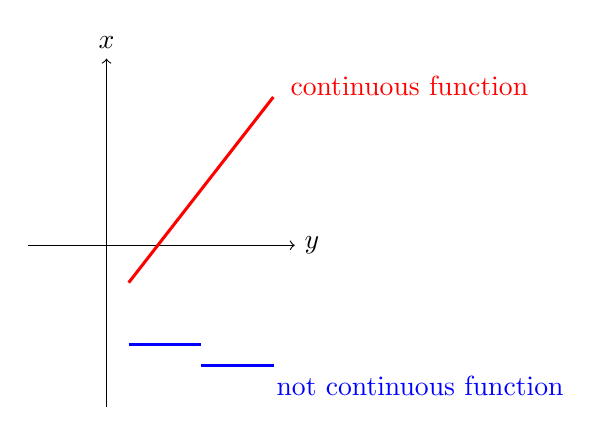
\begin{tikzpicture}[x=0.75pt,y=0.75pt,yscale=-1,xscale=1]
    %Straight Lines [id:da24929647938311184] 
    \draw  [->]  (189.3,210) -- (189.3,42.05) node[above] {$x$};
    %Straight Lines [id:da4428013785785254] 
    \draw  [->]  (151.6,132) -- (280,132) node[right] {$y$};
    %Straight Lines [id:da03148052252332034] 
    \draw[red,line width=1.1pt]  (200,150) -- (269.7,60.55) ;
    %Straight Lines [id:da8135470928175486] 
    \draw[blue,line width=1.1pt]    (200,180) -- (235,180) ;
    \draw[blue,line width=1.1pt]    (235,190) -- (270,190) ;
    %\draw[dashed]    (235,180) -- (235,190) ;
    
    % Text Node
    \draw[red] (276.7,49.2) node [anchor=north west][inner sep=0.75pt]    {continuous function};
    % Text Node
    \draw[blue] (270,193.7) node [anchor=north west][inner sep=0.75pt]    {not continuous function};
\end{tikzpicture} 
\subsection{Definition}
\begin{enumerate}[label=\protect\circled{\arabic*}]
    \item $f$ continuous at $a \in I$: \\ we say $f$ is continuous at $a$ - $a$ being a point of $I$ - if and only if:
    \begin{align*}
        f(a) &= \lim_{x \to a} f(x) \\
        f(a) &= \lim_{\begin{smallmatrix}
            x \to a \\
            x > a
        \end{smallmatrix}}f(x) = \lim_{\begin{smallmatrix}
            x \to a \\
            x < a
        \end{smallmatrix}}f(x) 
    \end{align*}
    \item $f$ continuous over $I$: \\ we say $f$ is continuous over $I \subset R$ if and only if $\forall a \in I$,$f$ is continuous at $a$
\end{enumerate}
\end{document}